% FiCRNN, figure 1: detailed view of one time step
\documentclass[border=8pt]{standalone}
\usepackage{amsmath,amssymb}
\usepackage{tikz}
\usetikzlibrary{positioning,arrows.meta,fit,backgrounds,calc}

\definecolor{cIn}{HTML}{E8EEF7}     \definecolor{cInD}{HTML}{3B5B8C}
\definecolor{cCnn}{HTML}{E6F2EA}    \definecolor{cCnnD}{HTML}{2E7D4F}
\definecolor{cFilm}{HTML}{FCEBDD}   \definecolor{cFilmD}{HTML}{C0622B}
\definecolor{cRnn}{HTML}{EFE7F6}    \definecolor{cRnnD}{HTML}{6A4C93}
\definecolor{cHead}{HTML}{F3F3F3}   \definecolor{cHeadD}{HTML}{555555}

\begin{document}
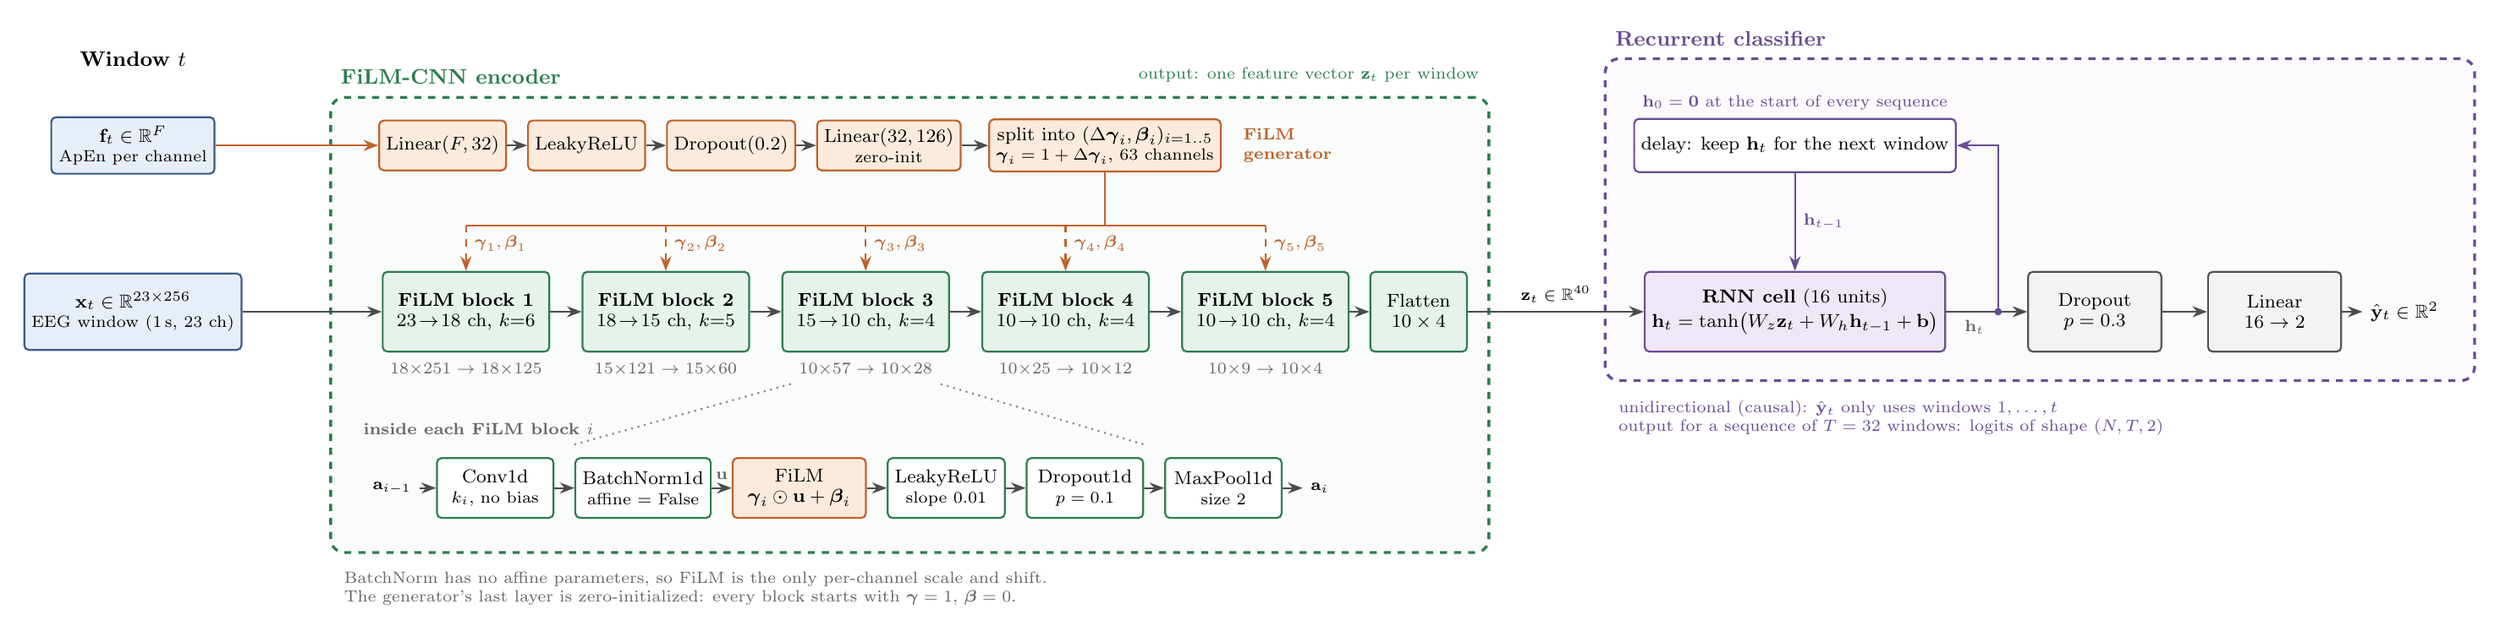
\begin{tikzpicture}[
  font=\footnotesize,
  >={Stealth[length=2.2mm]},
  arr/.style={->, thick, draw=black!70},
  filmarr/.style={->, thick, draw=cFilmD, dashed},
  box/.style={draw, rounded corners=2pt, thick, align=center, inner sep=3pt},
  inp/.style={box, draw=cInD, fill=cIn},
  film/.style={box, draw=cFilmD, fill=cFilm, minimum height=0.75cm},
  blk/.style={box, draw=cCnnD, fill=cCnn, minimum width=2.5cm, minimum height=1.2cm},
  op/.style={box, draw=cCnnD, fill=white, minimum height=0.9cm, minimum width=1.75cm},
  rnn/.style={box, draw=cRnnD, fill=cRnn, minimum width=2.1cm, minimum height=0.8cm},
  head/.style={box, draw=cHeadD, fill=cHead, minimum width=2.0cm, minimum height=0.8cm},
  dimlab/.style={font=\scriptsize\itshape, text=black!60},
  note/.style={font=\scriptsize, align=left},
]

\def\yg{1.6}    % FiLM generator row
\def\yb{-0.9}   % FiLM block row
\def\yz{-3.55}  % zoomed block row


\def\yg{1.6}    % FiLM generator row
\def\yb{-0.9}   % FiLM block row
\def\yz{-3.55}  % zoomed block row

% =====================================================================
% INPUTS FOR ONE WINDOW (left)
% =====================================================================
\node[inp, minimum width=2.45cm, minimum height=1.15cm] (xs0) at (0.45, \yb)
  {$\mathbf{x}_t\in\mathbb{R}^{23\times256}$\\[-1pt]{\scriptsize EEG window (1\,s, 23 ch)}};
\node[inp, minimum width=2.45cm, minimum height=0.85cm] (fs0) at (0.45, \yg)
  {$\mathbf{f}_t\in\mathbb{R}^{F}$\\[-1pt]{\scriptsize ApEn per channel}};
\node[font=\small\bfseries, align=center] at (0.45, \yg+1.3) {Window $t$};

% =====================================================================
% SHARED FiLM-CNN ENCODER (center)
% =====================================================================
\node[film] (g1) at (5.1, \yg) {Linear$(F,32)$};
\node[film, right=0.3cm of g1] (g2) {LeakyReLU};
\node[film, right=0.3cm of g2] (g3) {Dropout(0.2)};
\node[film, right=0.3cm of g3] (g4) {Linear$(32,126)$\\[-1pt]{\scriptsize zero-init}};
\node[film, right=0.4cm of g4] (g5) {split into $(\Delta\boldsymbol\gamma_i,\boldsymbol\beta_i)_{i=1..5}$\\[-1pt]{\scriptsize $\boldsymbol\gamma_i=1+\Delta\boldsymbol\gamma_i$, 63 channels}};
\foreach \a/\b in {1/2,2/3,3/4,4/5}{\draw[arr] (g\a) -- (g\b);}
\draw[arr, draw=cFilmD] (fs0.east) -- (g1.west);
\node[font=\scriptsize\bfseries, text=cFilmD, anchor=west, align=left] at ($(g5.east)+(0.2,0)$) {FiLM\\generator};

\foreach \i/\cin/\cout/\k/\lc/\lp [count=\n] in
  {1/23/18/6/251/125, 2/18/15/5/121/60, 3/15/10/4/57/28, 4/10/10/4/25/12, 5/10/10/4/9/4}{
  \node[blk] (B\i) at ({5.45+(\n-1)*3.0}, \yb)
    {\textbf{FiLM block \i}\\[-1pt]$\cin\!\to\!\cout$ ch, $k{=}\k$};
  \node[dimlab, below=1pt of B\i] (Bs\i) {$\cout{\times}\lc \to \cout{\times}\lp$};
}
\node[box, draw=cCnnD, fill=cCnn, minimum width=1.45cm, minimum height=1.2cm] (flat)
  at (19.75, \yb) {Flatten\\[-1pt]$10\times4$};
\draw[arr] (xs0.east) -- (B1.west);
\foreach \a/\b in {1/2,2/3,3/4,4/5}{\draw[arr] (B\a) -- (B\b);}
\draw[arr] (B5) -- (flat);

\coordinate (bus) at (0, {(\yg+\yb)/2+0.05});
\draw[thick, draw=cFilmD] (g5.south) -- (g5.south |- bus);
\draw[thick, draw=cFilmD] (B1.north |- bus) -- (B5.north |- bus);
\foreach \i in {1,...,5}{
  \draw[filmarr] (B\i.north |- bus) -- node[right, font=\scriptsize, text=cFilmD, pos=0.4]
    {$\boldsymbol\gamma_{\i},\boldsymbol\beta_{\i}$} (B\i.north);
}

% zoom into one block
\node[font=\scriptsize, anchor=east] (ain) at (4.75, \yz) {$\mathbf{a}_{i-1}$};
\node[op, anchor=west] (o1) at (5.0, \yz) {Conv1d\\[-1pt]{\scriptsize $k_i$, no bias}};
\node[op, right=0.3cm of o1] (o2) {BatchNorm1d\\[-1pt]{\scriptsize affine = False}};
\node[op, right=0.3cm of o2, draw=cFilmD, fill=cFilm, minimum width=2.0cm] (o3)
  {FiLM\\[-1pt]$\boldsymbol\gamma_i\odot\mathbf{u}+\boldsymbol\beta_i$};
\node[op, right=0.3cm of o3] (o4) {LeakyReLU\\[-1pt]{\scriptsize slope 0.01}};
\node[op, right=0.3cm of o4] (o5) {Dropout1d\\[-1pt]{\scriptsize $p=0.1$}};
\node[op, right=0.3cm of o5] (o6) {MaxPool1d\\[-1pt]{\scriptsize size 2}};
\node[font=\scriptsize, right=0.3cm of o6] (aout) {$\mathbf{a}_{i}$};
\draw[arr] (ain) -- (o1);
\draw[arr] (o1) -- (o2);
\draw[arr] (o2) -- node[above, dimlab] {$\mathbf{u}$} (o3);
\foreach \a/\b in {3/4,4/5,5/6}{\draw[arr] (o\a) -- (o\b);}
\draw[arr] (o6) -- (aout);
\begin{scope}[on background layer]
  \node[fit=(ain)(o1)(o6)(aout), draw=black!45, dotted, thick, rounded corners=3pt,
        inner sep=5pt, fill=white] (zoom) {};
\end{scope}
\node[font=\scriptsize\bfseries, text=black!60, anchor=south west] at ($(zoom.north west)+(0.05,0.02)$)
  {inside each FiLM block $i$};
\draw[black!45, dotted, thick] (Bs3.south west) -- (zoom.north west -| o2.west);
\draw[black!45, dotted, thick] (Bs3.south east) -- (zoom.north east -| o5.east);

\begin{scope}[on background layer]
  \node[fit=(g1)(g5)(B1)(flat)(zoom)(Bs1), draw=cCnnD, dashed, very thick,
        rounded corners=6pt, inner sep=9pt, fill=cCnn!25] (enc) {};
\end{scope}
\node[font=\small\bfseries, text=cCnnD, anchor=south west] at ($(enc.north west)+(0.05,0.05)$)
  {FiLM-CNN encoder};
\node[font=\scriptsize, text=cCnnD, anchor=south east] at ($(enc.north east)+(-0.05,0.08)$)
  {output: one feature vector $\mathbf{z}_t$ per window};

% =====================================================================
% RECURRENT CLASSIFIER (right)
% =====================================================================
\node[box, draw=cRnnD, fill=cRnn, minimum height=1.2cm] (rnn) at (25.4, \yb)
  {\textbf{RNN cell} (16 units)\\[1pt]
   $\mathbf{h}_t=\tanh\!\big(W_{z}\mathbf{z}_t+W_{h}\mathbf{h}_{t-1}+\mathbf{b}\big)$};
\node[head, minimum height=1.2cm] (dp) at (29.9, \yb) {Dropout\\[-1pt]$p=0.3$};
\node[head, minimum height=1.2cm] (lin) at (32.6, \yb) {Linear\\[-1pt]$16\to2$};
\node (yt) at (34.55, \yb) {$\hat{\mathbf{y}}_t\in\mathbb{R}^{2}$};
\draw[arr] (flat.east) -- node[above, font=\scriptsize] {$\mathbf{z}_t\in\mathbb{R}^{40}$} (rnn.west);
\coordinate (br) at (28.45, \yb);
\draw[arr] (rnn.east) -- node[pos=0.35, below, dimlab] {$\mathbf{h}_t$} (dp.west);
\draw[arr] (lin) -- (yt);
\draw[arr] (dp) -- (lin);
% recurrence loop
\node[box, draw=cRnnD, fill=white, minimum height=0.8cm] (delay) at (25.4, \yg)
  {delay: keep $\mathbf{h}_t$ for the next window};
\fill[cRnnD] (br) circle (1.6pt);
\draw[arr, draw=cRnnD] (br) |- (delay.east);
\draw[arr, draw=cRnnD] (delay.south) -- node[right, font=\scriptsize, text=cRnnD] {$\mathbf{h}_{t-1}$} (rnn.north);
\node[font=\scriptsize, text=cRnnD, anchor=south] (h0n) at (delay.north) {$\mathbf{h}_0=\mathbf{0}$ at the start of every sequence};
\begin{scope}[on background layer]
  \node[fit=(rnn)(delay)(h0n)(yt)(lin), draw=cRnnD, dashed, very thick, rounded corners=6pt,
        inner sep=12pt, fill=cRnn!20] (rc) {};
\end{scope}
\node[font=\small\bfseries, text=cRnnD, anchor=south west] at ($(rc.north west)+(0.05,0.05)$)
  {Recurrent classifier};
\node[note, text=cRnnD, anchor=north west] at ($(rc.south west)+(0.1,-0.15)$)
  {unidirectional (causal): $\hat{\mathbf{y}}_t$ only uses windows $1,\dots,t$\\
   output for a sequence of $T=32$ windows: logits of shape $(N,T,2)$};

\node[note, text=black!60, anchor=north west] at ($(enc.south west)+(0.1,-0.15)$)
  {BatchNorm has no affine parameters, so FiLM is the only per-channel scale and shift.\\
   The generator's last layer is zero-initialized: every block starts with $\boldsymbol\gamma=1$, $\boldsymbol\beta=0$.};

\end{tikzpicture}
\end{document}
